\documentclass[10pt,a4paper]{article}
\usepackage[utf8]{inputenc}
\usepackage[portuguese]{babel}
\usepackage[T1]{fontenc}
\usepackage{amsmath}
\usepackage{amsfonts}
\usepackage{amssymb}
\usepackage{graphicx}
\usepackage[portuguese]{algorithm2e}
\usepackage{comment}
\usepackage{hyperref}
\usepackage[all]{hypcap}
\usepackage{listings}
\usepackage{lstautogobble}
\usepackage[margin=2.2cm]{geometry}

\makeatletter	% let the hacks begin
\newcommand{\nosemic}{\renewcommand{\@endalgocfline}{\relax}}	% Drop semi-colon ;
\makeatother

\author{Gonçalo Ribeiro e Ricardo Amendoeira}
\title{Encaminhamento Inter-Domínio}
\begin{document}

\begin{titlepage}

	\begin{center}

		
\includegraphics[width=6cm]{./logoIST}\\[2.5cm]

		\textsc{\LARGE Algoritmia e Desempenho\\[5mm]
		em Redes de Computadores}\\[2cm]

		{ \huge \bfseries Conectividade em Digrafos \\[2.5cm] }


		\noindent
		\begin{center} \Large
			Gonçalo Ribeiro, 73294\\[5mm]

			Ricardo Amendoeira, 73373\\[4.5cm]

			\textit{Docente: Prof. João Luís Sobrinho}

		\end{center}

		\vfill

		{\large 9 de Dezembro de 2014}


	\end{center}

\end{titlepage}
\pagebreak

\section{Procura de Rota AS-AS}
O primeiro problema que nos é colocado é encontrar a rota que um sistema autónomo (AS) usa para chegar a outro. As únicas rotas possíveis são de um de três tipos: \textit{provider path}, \textit{peer path} ou \textit{costumer path}. Um AS prefere sempre uma rota de cliente a uma de par, uma de par a uma de fornecedor e uma de cliente a uma de fornecedor.

Pensámos e implementámos diversos algoritmos. Começámos por implementar um algoritmo DFS (depth-first search) que descobria todas as rotas permitidas da origem para o destino e após isso transformava as rotas numa string de 1's, 2's e 3's que eram depois ordenadas lexicograficamente de forma a descobrir qual a rota mais vantajosa em termos de tipo de caminho usado, tamanho do caminho e número de nós de cada tipo existentes no caminho. Embora esta solução funcionasse perfeitamente notámos que era computacionalmente dispendiosa pelo que decidimos descobrir um melhor algoritmo.

Pensámos então em implementar o algoritmo de procura com base numa BFS (breadth-first search) com restrições. Com uma BFS quando o algoritmo chega ao nó de destino sabemos que o caminho descoberto tem seguramente o comprimento mínimo. No entanto devido às restrições impostas pelo tipo de caminhos que são permitidos traz alguns problemas. Veja-se por exemplo a rede da Figura~\ref{fig:11}. Considere-se que corremos uma BFS com a restrição de que um nó a que se tenha chegado através de um fornecedor não pode explorar os seus fornecedores. Neste caso se tivermos o nó 4 como origem e 1 como destino o que ocorre é que 4 encontra 3 e 2, que marca como usados. 2 não pode continuar para 1 e 3 já está usado. Quando 3 tenta usar 2 para chegar a 1 (o que é legítimo) vê que 2 já está marcado e portanto pára e 1 não é encontrado. Ou seja a BFS restringida a seguir apenas caminhos válidos e nós não visitados pode não encontrar o destino quando efectivamente existe uma rota válida.

A nossa solução final é baseada numa BFS mas que não é tão \textit{greedy}. O algoritmo pode ser implementado recursivamente e a ideia base é um nó visitar primeiro todos os seus caminhos de cliente, depois todos os seus caminhos de par e por fim todos os seus caminhos de fornecedor, sendo que cada nó é usado apenas uma vez. O algoritmo é apresentado em mais pormenor no Algoritmo~\ref{algo:findroute}.

Note-se que o algoritmo não pode parar mal chegue ao destino porque não é garantido que o melhor caminho seja o primeiro a ser descoberto. Para além disso há que notar que para evitar o problema de um nó ser marcado como inutilizável quando ainda vai ser preciso para chegar ao destino passámos a marcar o nó como inutilizável apenas quando é visitado por um cliente.

\begin{figure}[h]
\centering
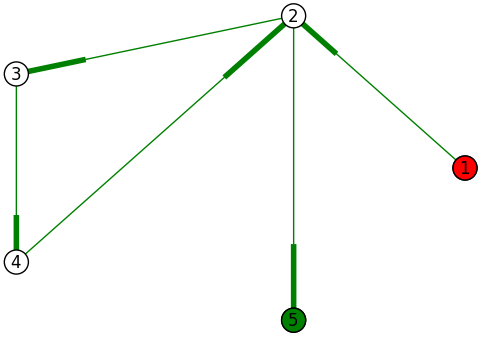
\includegraphics[scale=0.5]{11}
\caption{grafo do ficheiro 11.txt}
\label{fig:11}
\end{figure}


\lstset{emph={new_fringe, relation, neighbour, relation, node, explore, fringe, dest}, emphstyle=\itshape} 
\begin{algorithm}[H]
\caption{algoritmo que encontra a melhor rota AS-AS}
\label{algo:findroute}
\begin{lstlisting}
fringe = {origin}
findroute(dest, explore, fringe):

  if fringe is empty:
    return

  new_fringe = {}

  for each relation in explore:
    for each node in fringe:

      if node == dest:
        if this route is best than the elected route:
          elect this route

      for each neighbour who has relation:
        if neighbour is unvisited
              or (neighbour is a provider
              and has not been visited as a provider):
          mark neighbour as visited by node,
              who has relation to it
          add neighbour to new_fringe

    if relation is provider:
      findroute(dest, {costumers, peers, providers},
                new_fringe)
    else:
      findroute(dest, {costumers}, new_fringe)
    new_fringe = {}
\end{lstlisting}

\end{algorithm}


\section{Estatísticas da Rede}
Nesta parte o objectivo é fazer um programa que recolha estatísticas de uma rede, nomeadamente que conte o número de caminhos de cada um dos três tipos. Para resolver este problema estudámos vários algoritmos na esperança de que algum resultasse num implementação mais eficiente do que correr N vezes o Algoritmo~\ref{algo:findroute}. No entanto, não encontrámos uma solução significativamente melhor do que essa. Ainda assim notámos uma optimização que pode ser feita: quando uma rede é policy connected temos certeza de que um nó consegue chegar a todos os outros nós. Sendo assim, numa rede policy connected um nó que não tenha nem clientes nem pares garantidamente consegue chegar a todos os outros nós por meio de caminhos de fornecedor. Isso faz com que quando se encontra um nó nestas condições não seja necessário correr o Algoritmo~\ref{algo:findroute}.

Por falta de tempo não foi possível chegar a uma implementação satisfatória para gerar as estatísticas, a actual tem problemas com redes que contenham ciclos (embora em princípio esta topologia não aconteça no mundo real). Usar o Algoritmo~\ref{algo:findroute} daria os resultados correctos para qualquer topologia mas ao custo de um grande aumento na complexidade. Foi também tentada uma implementação do algoritmo de Floyd-Warshal adaptado para calcular os caminhos mais ``largos'' (em que rotas por clientes seriam consideradas mais largas que rotas por pares ou fornecedores e por pares mais largas que por fornecedores) e embora funcionasse e tivesse uma complexidade boa para o problema, a criação da matriz de dimensões N$\times$N para as maiores redes fornecidas pelo professor atingiam o limite de memória e portanto tornava o algoritmo inutilizável.


\section{Redes \textit{Policy Connected}}
Uma rede \textit{policy connected} é uma em que cada nó tem uma rota legal para todos os outros. Um nó tem sempre uma rota legal para os seus clientes e para os clientes dos seus pares. Facilmente se percebe que para que haja uma rota legal de cada nó para todos os outros é preciso que os nós Tier-1 estejam ligados entre si (por relações de par). Sendo assim é fácil escrever um algoritmo que verifique se a rede é policy connected. Esse algoritmo é o Algoritmo~\ref{algo:testpolicy}.

\lstset{emph={tier1, node, graph}, emphstyle=\itshape}
\begin{algorithm}
\caption{algoritmo que verifica se uma rede é policy connected}
\label{algo:testpolicy}
\begin{lstlisting}
is_policy_connected(graph):
  tier1 = {}

  for each node in graph:
    if node has no providers:
      add node to tier1

  for each node in tier1:
    if tier1 is not in {node.peers} union with {node}
      return False

  return True
\end{lstlisting}
\end{algorithm}


\section{Visualizador de Grafos}
Ao longo deste projecto criámos alguns grafos para melhor podermos testar as várias partes do projecto. De forma a podermos visualizar mais facilmente os grafos criados desenvolvemos em Python um \textit{script} que dado um ficheiro que descreve uma rede cria uma representação gráfica dessa rede.

Nos grafos criados por este programa os nós Tier-1 são marcados a vermelho e os nós que não têm nem pares nem clientes são marcados a verde. Os restantes nós são marcados a branco. A preto são desenhadas as arestas que indicam relações de pares e a verde as arestas que apontam para clientes. A direcção da aresta é representada por uma linha mais grossa no lado da cabeça da aresta.

Uma das redes fornecida pelo professor pode ser vista na Figura~\ref{fig:SmallNetwork}, tal como gerada pelo programa.

\begin{figure}[h]
\centering
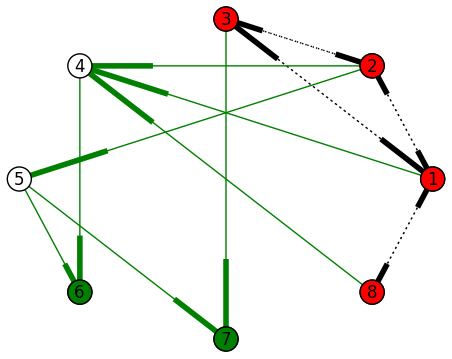
\includegraphics[scale=0.6]{SmallNetwork}
\caption{figura criada automaticamente a partir de SmallNetwork.txt}
\label{fig:SmallNetwork}
\end{figure}


\end{document}
